\section{Introduction}

Deep Neural Networks (DNNs) are extremely powerful machine learning
models that achieve excellent performance on difficult problems such
as speech recognition \cite{hinton12,dahl12b} and visual object
recognition \cite{kriz12,ciresan12,lecun98,le12}.  DNNs are
powerful because they can perform arbitrary parallel computation for a
modest number of steps.  A surprising example of the power of DNNs is
their ability to sort $N$ \!\!\!\!\quad $N$-bit numbers using only 2
hidden layers of quadratic size \cite{razborov}. So, while neural
networks are related to conventional statistical models, they learn an
intricate computation.  Furthermore, large DNNs can be trained with
supervised backpropagation whenever the labeled training set has
enough information to specify the network's parameters.  Thus, if
there exists a parameter setting of a large DNN that achieves good
results (for example, because humans can solve the task very rapidly),
supervised backpropagation will find these parameters and solve the
problem.

Despite their flexibility and power, DNNs can only be applied to
problems whose inputs and targets can be sensibly encoded with vectors
of fixed dimensionality.  It is a significant limitation, since many
important problems are best expressed with sequences whose lengths are
not known a-priori.  For example, speech recognition and machine
translation are sequential problems.  Likewise, question answering can
also be seen as mapping a sequence of words representing the question
to a sequence of words representing the answer.  It is therefore clear
that a domain-independent method that learns to map sequences to
sequences would be useful.

Sequences pose a challenge for DNNs because they require that the
dimensionality of the inputs and outputs is known and fixed.  
%%And
%%while Recurrent Neural Networks (RNNs) are natural candidates for this
%%task, they assume that there is a one-to-one correspondence between
%%the timesteps in the input and the output sequences, which is an
%%unrealistic assumption for most problems.
In this paper, we show that a straightforward application of the Long
Short-Term Memory (LSTM) architecture \cite{hochreiter97} can solve
general sequence to sequence problems.  The idea is to use one LSTM to
read the input sequence, one timestep at a time, to obtain large
fixed-dimensional vector representation, and then to use another LSTM
to extract the output sequence from that vector
(fig.~\ref{fig:translation-model2}).  The second LSTM is essentially a
recurrent neural network language model
\cite{rumelhart1986learning,mikolov2010recurrent,sundermeyer12} except
that it is conditioned on the input sequence.  The LSTM's ability to
successfully learn on data with long range temporal dependencies makes
it a natural choice for this application due to the considerable time
lag between the inputs and their corresponding outputs
(fig.~\ref{fig:translation-model2}).

There have been a number of related attempts to address the general
sequence to sequence learning problem with neural networks.   Our
approach is closely related to Kalchbrenner and Blunsom \cite{kal13} who were
the first to map the entire input sentence to vector, and is related 
to Cho et al.~\cite{cho14} although the latter was used only for rescoring hypotheses
produced by a phrase-based system.  Graves
\cite{graves13c} introduced a novel differentiable attention mechanism
that allows neural networks to focus on different parts
of their input, and an elegant variant of this idea was successfully
applied to machine translation by Bahdanau et al.~\cite{bog14}.  The Connectionist
Sequence Classification is another popular technique for mapping sequences
to sequences with neural networks, but it assumes a monotonic alignment
between the inputs and the outputs \cite{graves1}.


%% There have been a number of related attempts to address the general
%% sequence to sequence learning problem with neural networks.  The
%% Connectionist Sequence Classification technique uses a simple
%% HMM-transducer that assumes a monotonic alignment between the inputs
%% and the outputs \cite{graves1,graves2}.  More recently, Graves
%% \cite{graves13c} introduced a novel differentiable attention mechanism
%% that allows neural networks to sequentially focus on different parts
%% of the input, and an elegant variant of this idea was successfully
%% applied to machine translation by Bahdanau et al.~\cite{bog14}.  Our
%% approach is inspired by Kalchbrenner and Blunsom \cite{kal13} who were
%% the first to map the entire input sentence to vector, and is very similar
%% to Cho et al.~\cite{cho14} (although the model in this paper was
%% developed in parallel to Cho et al.~\cite{cho14}).  We will discuss
%% the relationship between the various approaches in section
%% \ref{sec:rel_work}.

\begin{figure}[h]
\centering 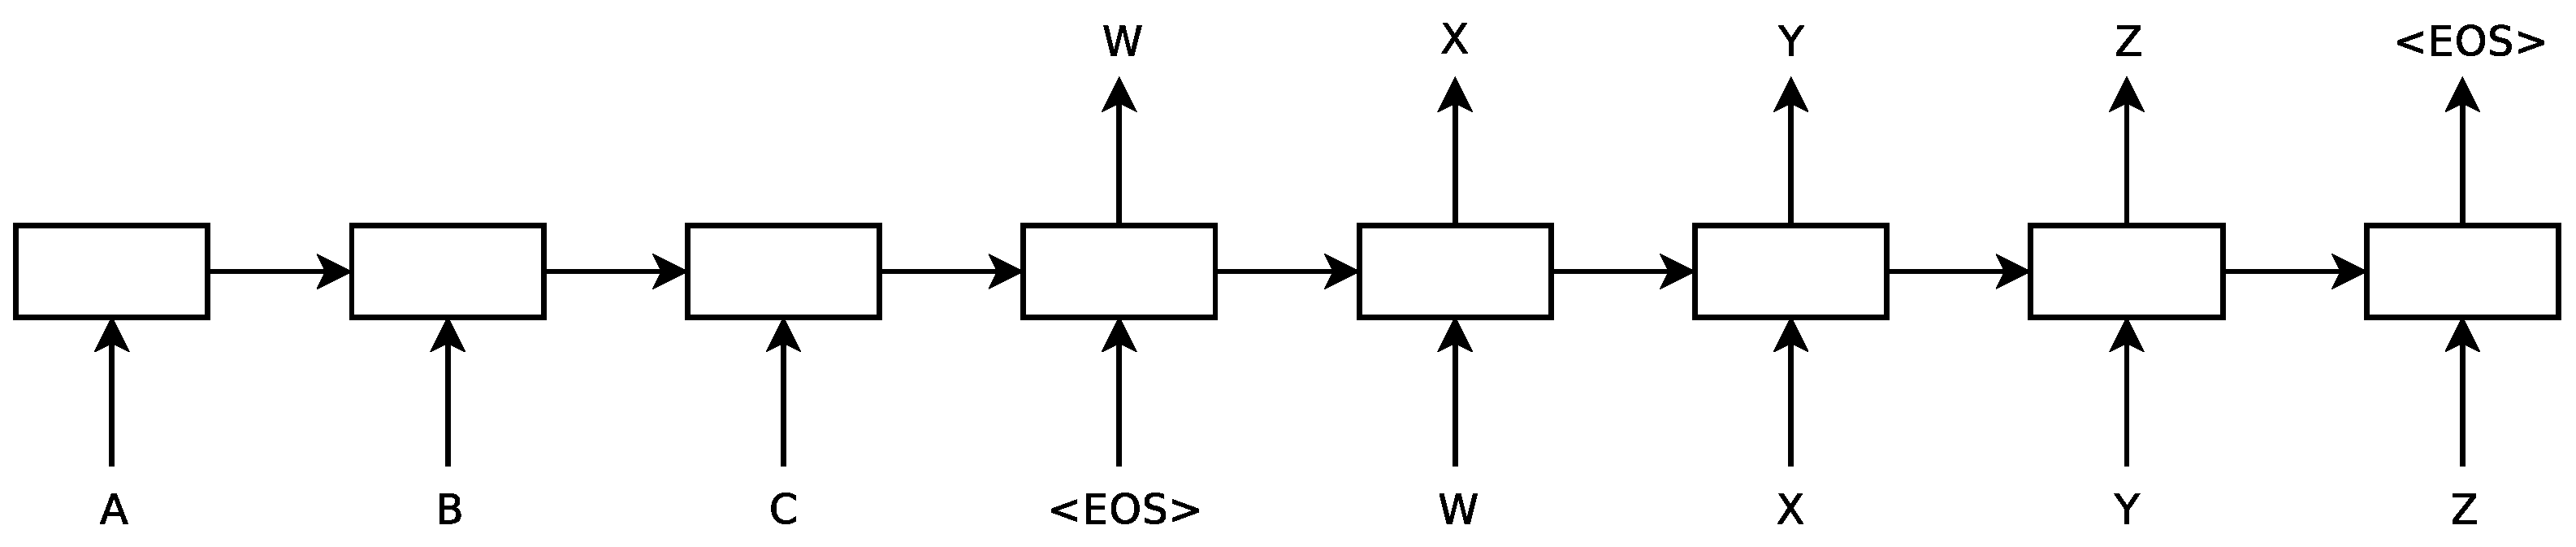
\includegraphics[width=0.9\textwidth]{Diagram1.eps}
\caption{\small Our model reads an input sentence ``ABC'' and produces
  ``WXYZ'' as the output sentence.  The model stops making predictions
  after outputting the end-of-sentence token.  Note that the LSTM
  reads the input sentence in reverse, because doing so introduces
  many short term dependencies in the data that make the optimization
  problem much easier. }
\label{fig:translation-model2}
\end{figure}

The main result of this work is the following.  On the WMT'14 English
to French translation task, we obtained a BLEU score of {\bf 34.81} by
directly extracting translations from an ensemble of 5 deep LSTMs
(with 384M parameters and 8,000 dimensional state each) using a simple left-to-right beam-search
decoder.  This is by far the best result achieved by direct
translation with large neural networks.  For comparison, the BLEU
score of an SMT baseline on
this dataset is 33.30 \cite{wmt14_en_fr}.  The
34.81 BLEU score was achieved by an LSTM with a vocabulary of 80k
words, so the score was penalized whenever the reference translation
contained a word not covered by these 80k.  This result shows that a
relatively unoptimized small-vocabulary neural network architecture which has much room
for improvement outperforms a phrase-based SMT system.

Finally, we used the LSTM to rescore the publicly available 1000-best
lists of the SMT baseline on the same task \cite{wmt14_en_fr}.  By
doing so, we obtained a BLEU score of 36.5, which improves the
baseline by 3.2 BLEU points and is close to the previous best published
result on this task (which is 37.0 \cite{durrani-EtAl:2014:W14-33}).

Surprisingly, the LSTM did not suffer on very long sentences, despite
the recent experience of other researchers with related architectures
\cite{curse}.  We were able to do well on long sentences because we
reversed the order of words in the source sentence but not the target
sentences in the training and test set. By doing so, we introduced
many short term dependencies that made the optimization problem much
simpler (see sec.~\ref{sec:model} and \ref{sec:rev_rev}).  As a result, SGD could learn
LSTMs that had no trouble with long sentences.  The simple trick of
reversing the words in the source sentence is one of the key technical
contributions of this work.
 
A useful property of the LSTM is that it learns to map an input
sentence of variable length into a fixed-dimensional vector
representation.  Given that translations tend to be paraphrases of the
source sentences, the translation objective encourages the LSTM to
find sentence representations that capture their meaning, as sentences
with similar meanings are close to each other while different
sentences meanings will be far. A qualitative evaluation supports
this claim, showing that our model is aware of word order and is
fairly invariant to the active and passive voice.

